\subsection{КМД-3}
\label{sec:cmd3}

\begin{figure}[htbp]
    \centering
    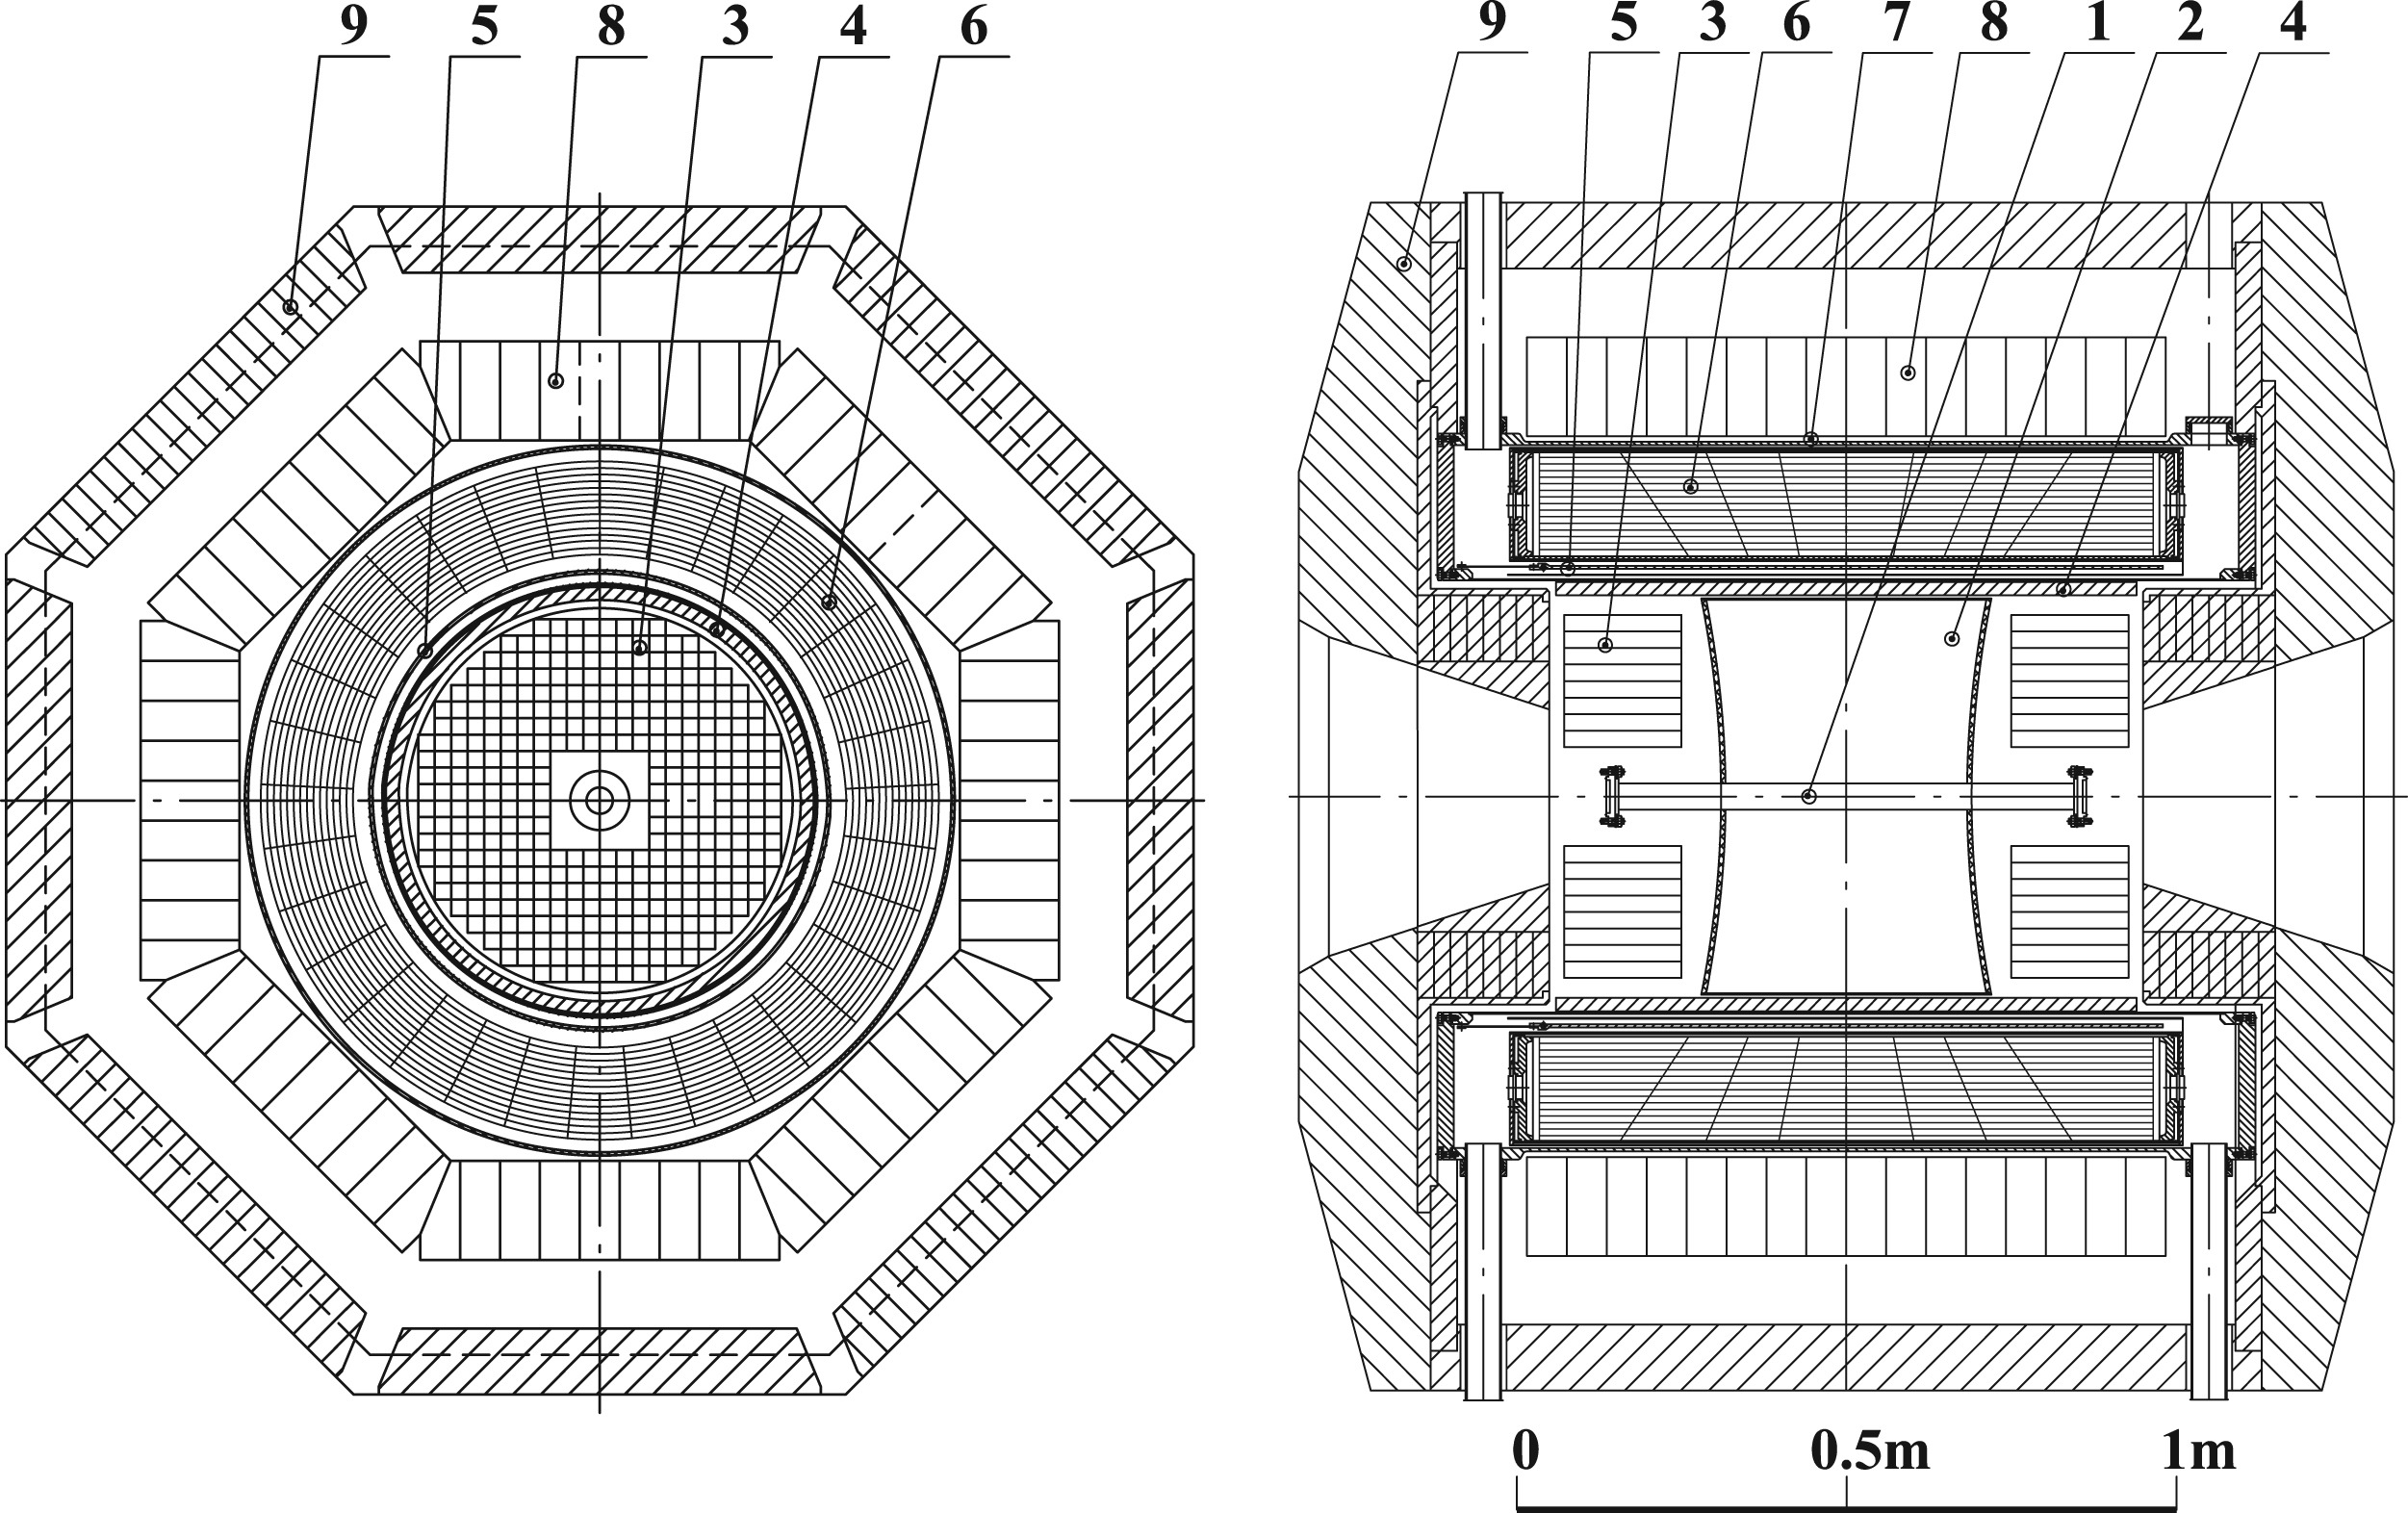
\includegraphics[width = .9\textwidth]{img/cmd3_detector/cmd3_layout.jpeg}
    \caption{Схема детектора КМД-3:
    	1 --- вакуумная труба,
    	2 --- дрейфовая камера,
    	3 --- \ce{BGO} калориметр,
    	4 --- Z-камера,
    	5 --- сверхпроводящий соленоид,
    	6 --- \ce{LXe} калориметр,
    	7 --- время-пролётная система,
    	8 --- \ce{CsI} калориметр,
    	9 --- ярмо магнита.
    }
    \label{fig:cmd3}
\end{figure}


Для проведения экспериментов на электрон-позитронном коллайдере \mbox{ВЭПП-2000} был частично модернизирован детектор СНД и создан новый универсальный детектор,
который получил название криогенного магнитного детектора третьего поколения
---
КМД-3 \cite{Khazin2010},
позволяющий регистрировать и измерять с высокой точностью параметры заряженных частиц и фотонов.
В период работы с 2011 года детектором КМД-3 было набаран интеграл светимости \SI{120}{\pbarnr^{-1}}.
Общий вид детектора представлен на Рис.~\ref{fig:cmd3}.
Электронные и позитронные пучки сталкиваются в центре вакуумной камеры (1), которая имеет внутренний диаметр \SI{34}{\mmr}. 
Центральная часть вакуумной камеры сделана из алюминия толщиной \SI{0.5}{\mmr} (\SI{5.3e-3}{\Xrad}\footnote{\si{\Xrad} --- радиационная единица длины.}) и длиной \SI{20}{\cmr}.

Для определения координат,
углов и импульсов заряженных частиц область столкновения пучков
охватывает трековая система,
которая находится внутри тонкого сверхпроводящего соленоида (толщина
\SI{0.18}{\Xrad},
магнитное поле \SI{1.3}{\teslaru}). 
Трековая система состоит из дрейфовой камеры,
Z-камеры и торцевого калориметра на основе кристаллов ортогерманата висмута \ce{Bi4Ge3O12}.
Вне магнитного поля в цилиндрической части детектора находятся жидко-ксеноновый калориметр \ce{LXe}(6)
и калориметр на основе активированных кристаллов \ce{CsI}(7). 
Жидко-ксеноновый калориметр позволяет измерить координаты точки конверсии фотона и совместно с калориметром на основе активированных кристаллов \ce{CsI} измерить энергию фотона.
Для фотонов, летящих из места встречи пучков, все три калориметра покрывают \SI{95}{\percent} телесного угла.
Между жидко-ксеноновом калориметром и \ce{CsI} калориметром расположена время-пролётная система (7).
Снаружи детектор окружен мюонной пробежной системой (8) на основе сцинтилляционных счётчиков для
подавления фона космических частиц.

%-----------------------------------
%	SUBSECTION Дрейфовая камера
%-----------------------------------

\subsubsection{Дрейфовая камера}
\label{sec:dc}

Дрейфовая камера (ДК) детектора КМД-3 способна работать при высоких загрузках и эффективно регистрировать многотрековые события, \cite{driftChCMD3Grancagnolo2010}. 
Координаты, углы и импульсы заряженных частиц измеряются в ДК,
которая плотно вставлена внутрь двухслойной многопроволочной пропорциональной Z-камеры (4). 
ДК представляет собой цилинидрический объём длиной \SI{44}{\cmr} и диаемтром \SI{60}{\cmr}.
Внутренняя и наружная цилиндрические оболочки,
а также торцевые фланцы сделаны из углепластика,
чтобы уменьшить количество пассивного вещества на пути частиц.
Торцевые фланцы выполенены в виде сегментов сферы.
Дрейфовая камера состоит из \num{1218} гексогональных ячеек с длиной диагонали \SI{18}{\mmr}.
Ячейка образована шестью полевыми проволочками с сигнальной проволочкой по центру.
Полевые проволочки имеют диаметр \SI{80}{\umr} и сделаны из титана, покрытого золотом. 
Сигнальные проволочки,
диаметром \SI{15}{\umr},
изготовлены из сплава вольфрам-кремний.
Камера продувается газовой смесью $\ce{Ar}:\ce{iC4H10}$ в пропорции $80:20$.
Суммарное количество вещества в ДК для частицы,
вылетевшей перпендикулярно по оношению к оси пучков,
эквиванлентно \SI{0.015}{\Xrad}.
Для частицы летящей вдоль оси $z$ из плоскости центрального сечения камеры
--- \SI{0.04}{\Xrad}.
Максимальное время дрейфа ионизации достигает \SI{600}{\nsr}.

Поперечные координаты трека измеряются по времени дрейфа первичной ионизации до сигнальных проволочек с точностью \SI{\sim 100}{\umr}.
Продольные координаты треков измеряются методом деления заряда и в среднем точность измерения составляет \SIrange{2}{3}{\mmr}. 

Поскольку камера расположена в магнитном поле,
в стандартном режиме работы \SI{1.3}{\teslaru},
то по кривизне треков заряженных частиц определяется их импульс и знак электрического заряда.

Абсолютная калибровка шкалы (пересчёт отношения зарядов на концах проволочки в продольную координату) осуществляется с использованием информации с Z-камеры,
которая имеет точность восстановления продольных координат трека \SI{\sim 0.5}{\mmr},
а систематическую погрешность меньше \SI{0.1}{\mmr}.
Импульсное разрешение ДК составило
$\sigma_p / p = \SIrange{1.3}{4.5}{\percent}$
для импульсов лежащих в диапазоне
\SIrange{160}{1000}{\MeVr \per \clight} (см. Рис.~\ref{fig:dc_mom_res}).
Разрешение по азимутальному углу равно \SI{9}{\mradianru} и \SI{3.5}{\mradianru}
для частиц с импульсами \SI{160}{\MeVr \per \clight} и \SI{1}{\GeVr \per \clight},
соответственно.
Разрешение по полярному углу практически не зависит от величины импульсы
и равно \SI{\sim 15}{\mradianru}.
Точность определения велечины удельных энергопотерь $\dif E / \dif x$
эквивалентна \SIrange{10}{13}{\percent}.
% Таким образом для частиц с импульсом \SI{500}{\MeVr \per \clight} разрешение составляет \SI{2.5}{\percent}


\begin{figure}
    \centering
    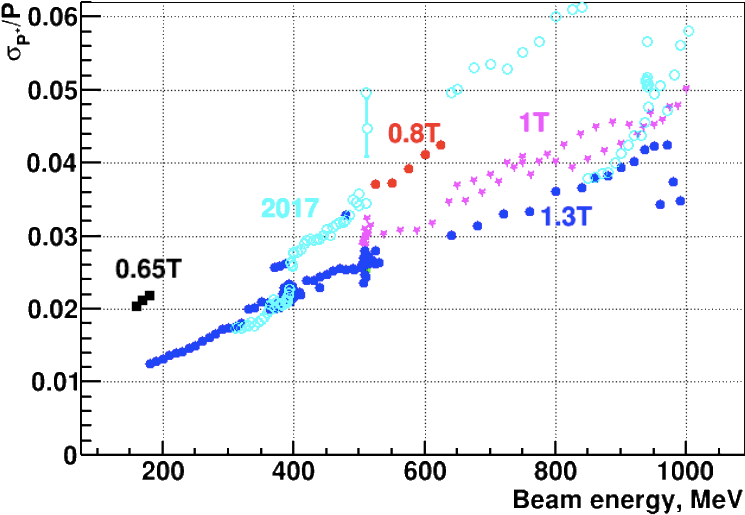
\includegraphics[height=.5\textwidth]{img/cmd3_detector/dc_mom_res.png}
    \caption{Импульсное разрешение дрейфовой камеры.}
    \label{fig:dc_mom_res}
\end{figure}


%-----------------------------------
%	SUBSECTION Z-камера
%-----------------------------------

\subsubsection{Z-камера}

Z-камера это двухслойная многопроволочная пропорциональная камера с анодным и катодным считыванием информации, \cite{Anashkin1992}.
Z-камера детектора КМД-3 является не только координатным детектором,
но и одним из основных элементов первичного заряженного триггера.
В каждом слое камеры \num{704} анодных проволочек, объединенных в $24$ сектора.
Камера продувается быстрой газовой смесью на основе фреона-14 \ce{CF4} и изобутана \ce{iC4H10} в пропорции $80:20$,
что позволяет достигнуть временной разброс анодных сигналов меньше \SI{5}{\nsr}.

Два слоя Z-камеры обеспечивают практически \SI{100}{\percent} эффективность регистрации заряженной частицы,
что особо важно для выроботки первичного сигнала заряженного триггера.
% Использование Z-камеры в первичном триггере предъявляет повышенные требования к ее эффективности.
% Наличие у камеры двух независимых слоёв позволяет обеспечить практически \SI{100}{\percent} эффективность запуска.
% Поскольку Z-камера расположена внутри цилиндрического калориметра, необходимо, чтобы она содержала минимальное количество вещества.
% Характерный масштаб задается толщиной сверхпроводящего магнита, составляющего основную массу вещества перед калориметром (примерно \SI{0.18}{\Xrad}).
Так как Z-камера находится перед цилиндрическим калориметро,
то во избежание ухудшения энергетического разрешения калориметра,
конструкция Z-камеры оптемизировалась по количеству используемого вещества и составила в среднем \SI{0.02}{\Xrad} для нормально падающей частицы,
что заметно меньше толщины сверхпроводящего соленоида (\SI{0.18}{\Xrad}),
находящегося также перед цилиндрическим калориметром.

%-----------------------------------
%	SUBSECTION Цилиндрический калориметр
%-----------------------------------

\subsubsection{Цилиндрический калориметр}
\label{sel:barrel_calorimeter}

Цилиндрический калориметр детектора КМД-3 состоит из двух слоёв и перекрывает полярные углы от \ang{38} до \ang{142},
охватывая \SI{79}{\percent} полного телесного угла,
\cite{BarrelCalCMD3Anisenkov:2013yva}.
Общая толщина активного вещества для нормально падающей частицы составляет \SI{13.3}{\Xrad}.
Внутренний слой представлен жидко-ксеноновым калориметром,
а внешний
---
кристаллическим калориметром на основе \ce{CsI(Na)} и \ce{CsI(Tl)}.

Толщина ближнего к оси пучков жидко-ксенонового калориметра составляет \SI{5.2}{\Xrad},
масса ксенона \num{1.2} тонны. 
Второй,
внешний калориметр построен на основе кристаллов \ce{CsI(Na)} и \ce{CsI(Tl)} общим числом \num{1152} и весом равен \num{2.2} тонны, 
радиационная длина \SI{8.1}{\Xrad}.

Суммарно перед активном веществом калориметра находится 
\SI{6.27}{\gr \per \cubed \cmr} или \SI{0.35}{\Xrad} пассивного вещества.
Между кристаллическим и жидким калориметром находится 
\SI{4.63}{\gr \per \cubed \cmr} или \SI{0.25}{\Xrad}.

Энергетическое разрешение цилиндрического калориметра для событий баба рассеяния описывается функцией
$\sigma_E^{\text{bar}} / E = \frac{ \SI{3.6}{\percent} }{ \sqrt{ E / \si{\GeVr} } } \oplus \SI{2.7}{\percent}$
(см. Рис.~\ref{fig:cal_energy_resolution}), \cite{Anisenkov:2017pgv}.
Пространственное разрешение цилиндрического калориметра для кластеров с восстановленной точкой конверсией по полоскам \ce{LXe} калориметра описывается функцией
$\sigma_{\varphi} / \si{\mradianru} = 3.70 + 0.33 / (0.25 + E / \si{\GeVr})$ (см. Рис.~\ref{fig:cal_spatial_resolution}).
В отсутствие полосковой информации
---
$\sigma_{\varphi} / \si{\mradianru} = 37.0 + 3.6 / (0.1 + E / \si{\GeVr})$.

% В соответствии с моделированием для $\gamma$-квантов с энергией \SI{350}{\MeVr} доля энергии,
% выделившейся в \ce{CsI} калориметре,
% составляет \SI{\sim 20}{\percent},
% для фотона с энергией \SI{950}{\MeVr}
% ---
% уже около \SI{30}{\percent}.

%-----------------------------------
%	SUBSUBSECTION Жидко-ксеноновый калориметр
%-----------------------------------

\paragraph{Жидко-ксеноновый калориметр}
\label{sec:lxe}

\begin{figure}[htbp]
    \begin{minipage}[t]{0.27\textwidth}
        \centering
        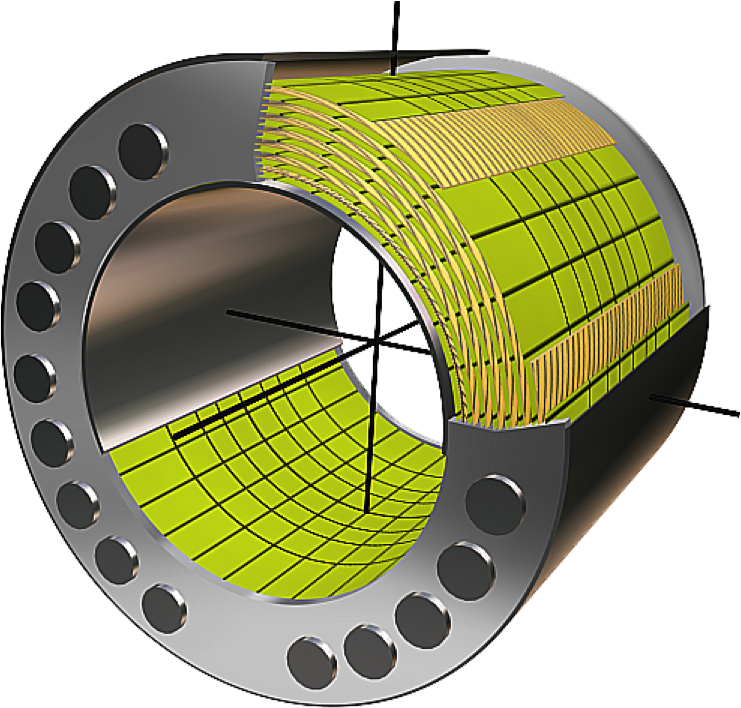
\includegraphics[width=\textwidth]{img/cmd3_detector/lxe_sketch.png}
        \label{fig:lxe_sketch}
        \caption{Жидкоксеноновый калориметр.}
    \end{minipage}
    \hfill
    \begin{minipage}[t]{0.68\textwidth}
        \centering
        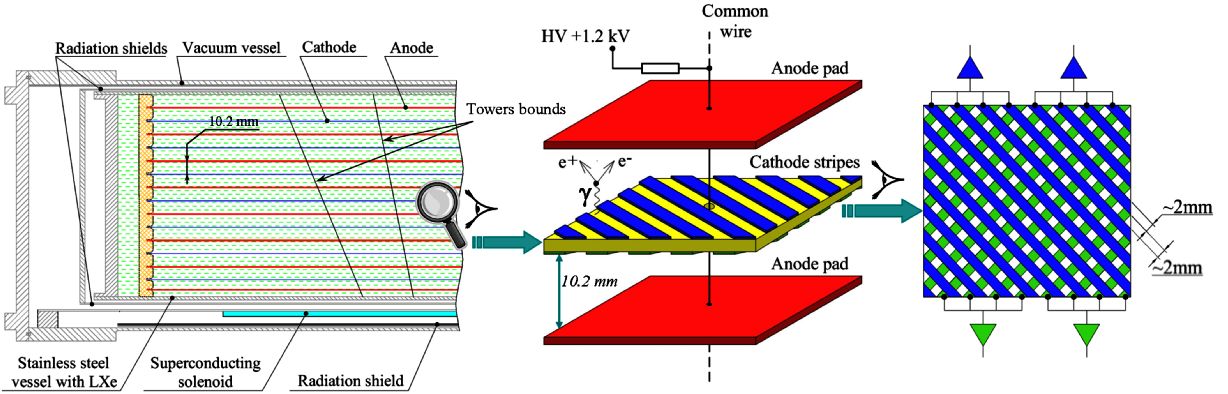
\includegraphics[width=\textwidth]{img/cmd3_detector/lxe_electrode_structure.png}
        \label{lxe_electrode_structure}
        \caption{Электроника жидкоксеновового калориметра.}
  \end{minipage}
\end{figure}

Жидко-ксеноновый калориметр показан на Рис.~\ref{fig:lxe_sketch},
и состоит из 15 соосных цилиндров,
семь из которых имеют полосковую структуру и являются катодами,
а восемь цилиндров образуют аноды.
Медная фольга каждого анода разделена на 8 колец вдоль оси пучка.
Каждое кольцо, в свою очередь,
поделено на \num{33} одинаковых сегмента в $R-\varphi$ плоскости. 
Образованные таким образом прямоугольники,
электрически соединены по радиусу и образуют башни в количестве \num{264}, каждая из которых смотрит на точку взаимодействия пучков.
Зазор между анодом и катодом \SI{10.2}{\mmr}.
% и при рабочем напряжении $\sim 1500$~В время дрейфа электронов составляет $\sim 4.5$~мкс.
Диаметры внутреннего и наружного цилиндров равны \SI{738}{\mmr} и \SI{1024}{\mmr} соответственно,
длина \SI{920}{\mmr}. 

Каждый катодный электрод на обоих сторонах разделен на полоски,
которые по отношению к оси пучков составляют углы \ang{\pm 45}. 
Каждая полоска, в свою очередь,
подразделена на 4 узких полоски шириной \SI{2}{\mmr} и зазором между ними \SI{2}{\mmr}. 
Такая структура полосок полупрозрачна и индуцированный сигнал практически одинаков на обеих сторонах катода. 
В результате обе координаты точки конверсии фотона могут быть измерены в одном зазоре.
Полное число катодных каналов \num{2124}.

Координатное разрешение измерялось по отобранным коллинеарным событиям,
используя аналоговую информацию с полосок. 
Координаты трека в каждом зазоре определяются методом центра тяжести,
через которые проводится оптимальная прямая
линия. 
В результате было показано,
что пространственное разрешение составляет \SIrange{\sim 1}{2}{\mmr}.


%-----------------------------------
%	SUBSUBSECTION Калориметр на основе кристаллов CsI
%-----------------------------------

\paragraph{Калориметр на основе кристаллов CsI}
\label{sec:csi}

\begin{figure}[htbp]
    \begin{minipage}[t]{0.35\textwidth}
        \centering
        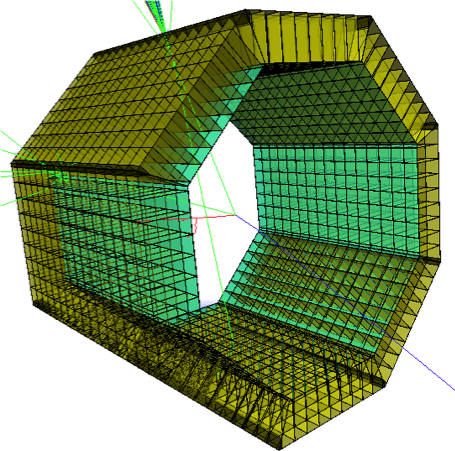
\includegraphics[width=\textwidth]{img/cmd3_detector/csi_scketch.png}
        \label{fig:lxe_sketch}
        \caption{\ce{CsI} калориметр.}
    \end{minipage}
    \qquad
    \begin{minipage}[t]{0.60\textwidth}
        \centering
        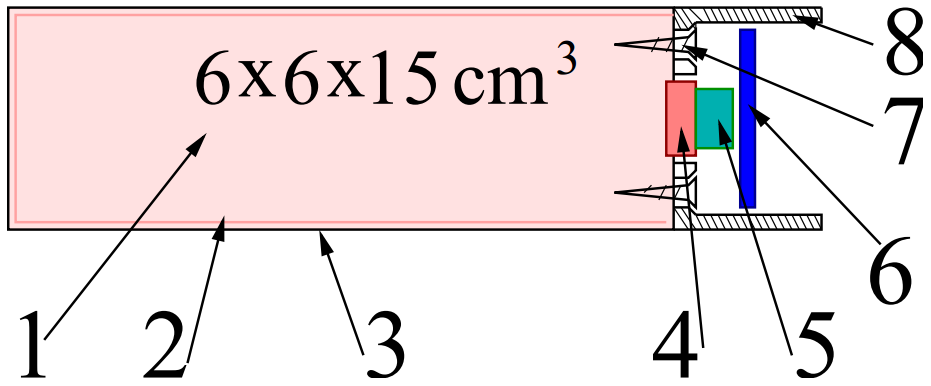
\includegraphics[width=.9\textwidth]{img/cmd3_detector/csi_crystal_scheme_v2.png}
        \label{lxe_electrode_structure}
        \caption{Счётчик \ce{CsI} калориметра:
        1 --- сцинтилляционный кристалл,
        2 --- белый пористый тефлон Gore-Tex,
        3 --- алюминизированный лавсан,
        4 --- pin-фотодиод,
        5 --- резиновый уплотнитель,
        6 --- предусилитель,
        7 --- шуруп,
        8 --- стальная рама.}
  \end{minipage}
\end{figure}


Калориметр на основе кристаллов \ce{CsI(Tl)} и \ce{CsI(Na)} состоит из 8 одинаковых октантов и каждый содержит 9 линейных модулей с \num{16} кристаллами, ориентированных вдоль оси пучков,
\cite{Aulchenko:2015msa}.
Зазор между кристаллами составляет не более \SI{0.5}{\mmr}.
Семь центральных модулей состоят из прямоугольных кристаллов с размерами $60 \times 60 \times \SI{150}{ \cubic\mmr}$.
Два боковых модуля имеют специальную форму кристаллов, чтобы обеспечить плотное сочленение двух соседних октантов без зазоров. 
Регистрация светового сигнала с каждого сцинтилляционного кристалла производится с помощью полупроводникового PIN фотодиода S2744-8 фирмы Hamamatsu Photonics с чувствительной площадью $1 \times \SI{2}{\square\cmr}$. 
Токовые сигналы с фотодиодов поступают на входы зарядочувствительных предусилителей,
размещённых непосредственно около фотодиодов и дающих на выходе парафазный сигнал.
По витой паре сигнал поступает на плату усилителей-формировщиков-оцифровщиков УФО-32,
способную обслуживать до двух линеек.
В плате после аттенюатора сигнал делится на две части.
Первая служит для выработки триггерного сигнала,
для чего в плате формируется \num{5} сигналов суммарного энерговыделения,
которые поступают на плату амплитудных дискриминаторов и сумматоров АДИС,
формирующих сигнал о срабатывание калориметра для последующего использования в триггере детектора.



\begin{figure}[htbp]
    \begin{minipage}[t]{0.475\textwidth}
        \centering
        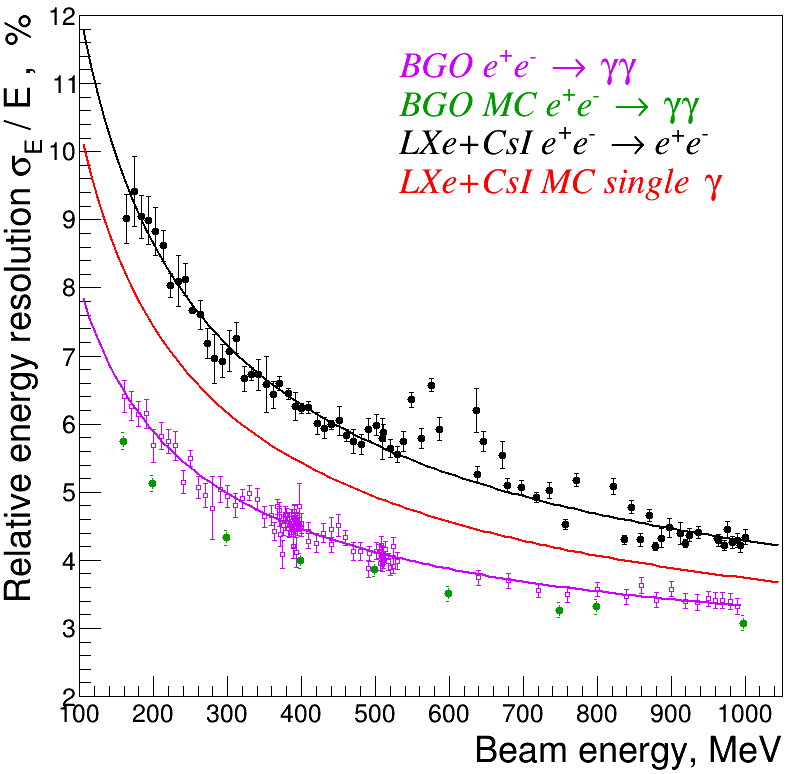
\includegraphics[width=\textwidth]{img/cmd3_detector/comb_energy_resolution.png}
        \label{fig:cal_energy_resolution}
        \caption{Энергетическое разрешение калориметров.}
    \end{minipage}
    \hfill
    \begin{minipage}[t]{0.475\textwidth}
        \centering
        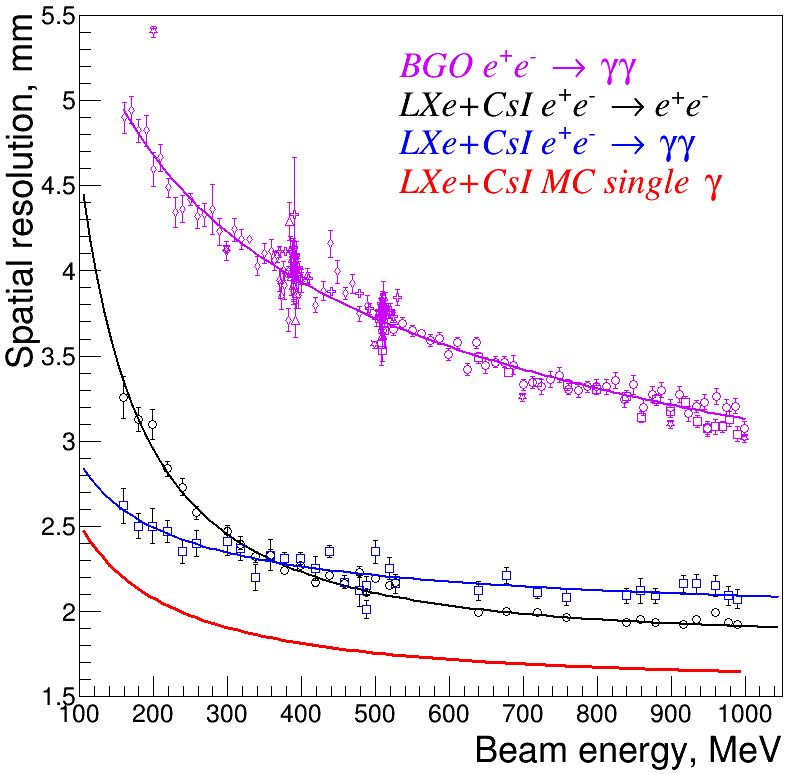
\includegraphics[width=\textwidth]{img/cmd3_detector/comb_spatial_resolution.png}
        \label{fig:cal_spatial_resolution}
        \caption{Пространственное разрешение калориметров.}
  \end{minipage}
\end{figure}



%-----------------------------------
%	SUBSECTION Торцевой калориметр на основе кристаллов BGO
%-----------------------------------

\subsubsection{Торцевой калориметр на основе кристаллов BGO}
\label{sec:bgo}

\begin{figure}[htbp]
    \begin{minipage}[t]{0.475\textwidth}
        \centering
        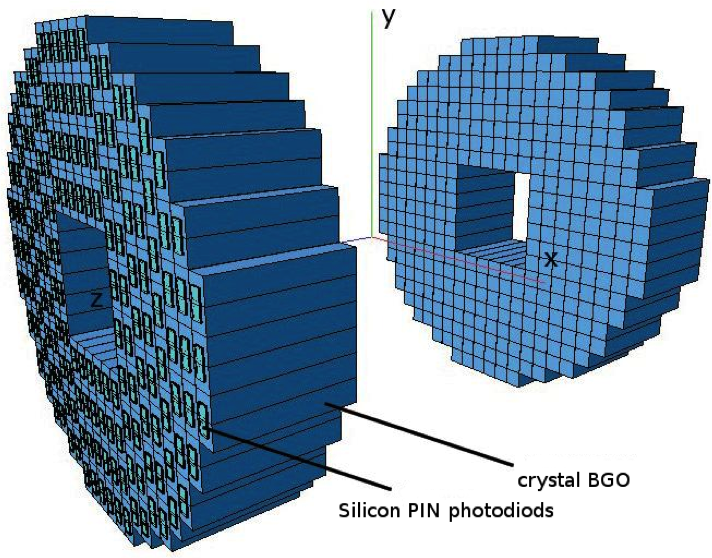
\includegraphics[width=\textwidth]{img/cmd3_detector/bgo_scetch.png}
        \label{fig:cal_energy_resolution}
        \caption{\ce{BGO} калориметр.}
    \end{minipage}
    \hfill
    \begin{minipage}[t]{0.475\textwidth}
        \centering
        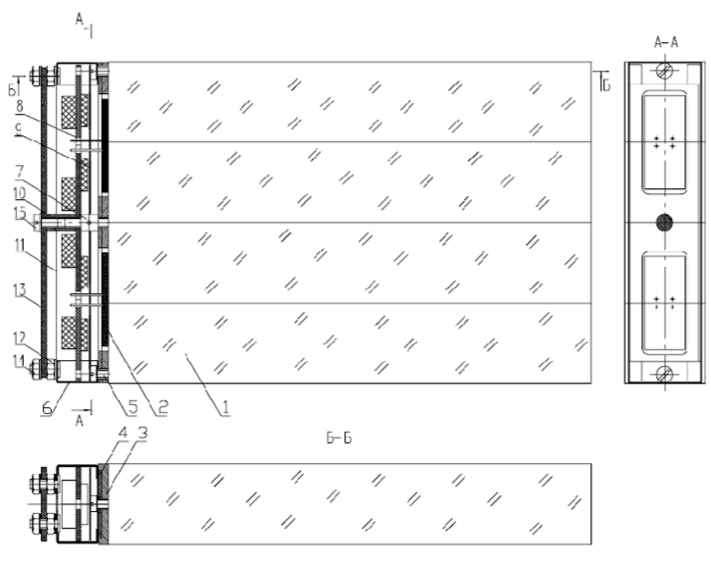
\includegraphics[width=\textwidth]{img/cmd3_detector/bgo_module_scheme.png}
        \label{fig:cal_spatial_resolution}
        \caption{Схема модуля \ce{BGO} калориметра.}
  \end{minipage}
\end{figure}

Торцевой калориметр на основе кристаллов ортогерманата висмута \ce{Bi4Ge3O12} (\ce{BGO}) представляет из себя два диска, расположенных вплотную к торцам ДК, \cite{BGOAkhmetshin2009}.
По центру этих дисков имеются отверстия для вакуумной камеры и компенсирующих магнитов.
Калориметр перекрывает полярные углы,
отсчитанные от оси пучков,
от \ang{16} до \ang{49} и от \ang{131} до \ang{164} и покрывает примерно \SI{30}{\percent} от полного телесного угла.
Для фотонов с энергиями 
\SIrange[range-phrase = --, range-units = single]{100}{700}{\MeVr}
энергетическое разрешение составляет 
\SIrange[range-phrase = --, range-units = single]{\sim 4}{8}{\percent},
а угловое разрешение \SI{\sim 0.02}{\radianru}.
Каждый диск состоит из \num{340} одинаковых кристаллов с размерами
\SI[product-units = power]{25 x 25 x 150}{\mmr}
и общим весом
\SI[product-units = single]{2 x 225}{\kgr}. 
Радиационная толщина калориметра для нормально падающих частиц составляет \SI{13.4}{\Xrad}.
Световой сигнал с каждого кристалла регистрируется полупроводниковым фотоприемниками S3590-08 фирмы Hamamatsu Photonics
с чувствительной областью \SI[product-units = power]{1 x 1}{\cmr},
имеющие высокую квантовую эффективность и стабильность в работе. 
Измерения показали,
что световыход составляет \SI{\sim 600}{\elementarycharge\per\MeVr},
а электронный шум \SI{\sim 500}{\elementarycharge},
что эквивалентно \SI{\sim 0.8}{\MeVr}.
Температура калориметра стабилизируется с помощью водного охлаждения.



%-----------------------------------
%	SUBSECTION Мюонная пробежная система
%-----------------------------------

\subsubsection{Мюонная пробежная система}
\label{sec:mu}

Мюонная пробежная система состоит из \num{36} сцинтилляционных счетчика и расположена с наружи магнитного ярма.
Мюоны с энергией больше \SI{550}{\MeVr},
рожденные в $e^+e^-$-столкновениях,
будут долетать до этих счетчиков. 
Каждый счетчик имеет размеры \SI[product-units = power]{2 x 20 x 150}{\cmr} и просматривается с каждой стороны двумя ФЭУ-84.
Сигналы с ФЭУ усиливаются и оцифровываются в платах TQ. 
На этой системе получено временное разрешение \SI{\sim 1}{\nsr}, что достаточно для подавления космических событий, имеющих время пролета через детектор \SI{\sim 7}{\nsr}.


%-----------------------------------
%	SUBSECTION Время-пролетные счетчики
%-----------------------------------

\subsubsection{Время-пролетные счетчики}
\label{sec:tof}

Время-пролетные счетчики [???], на основе сцинтиллятора ВС-406 фирмы <<БАЙКРОН>> расположены в
узком зазоре (\SI{7}{\mmr}) между ксеноновым и \ce{CsI} калориметрами и предназначены для регистрации продуктов
аннигиляции антинейтронов, рождающихся в реакции $e^+e^- \to n \bar{n}$. 
Всего \num{16} одинаковых счетчиков с размерами \SI[product-units = power]{0.5 x 20 x 90}{\cmr},
каждые два из которых крепятся на лицевой стороне \ce{CsI} калориметра,
образуя замкнутый октант.
Каждый счетчик просматривается двумя компактными фотоприемниками,
сделанных на основе микроканальных пластин
(МКП, диаметр --- \SI{30}{\mmr}, высота --- \SI{17}{\mmr}). 
Прямо на корпусе МКП смонтирован высоковольтный делитель и предусилитель с полосой пропускания \SI{\sim 1}{\GHzr}. 
Сигналы с МКП поступают на входы плат TQ (\num{16} каналов),
где они усиливаются и оцифровываются. 
На этой системе получено временное разрешение \SI{\sim 1}{\nsr}.




\subsubsection{Система запуска детектора}
\label{sec:trigger}

Система запуска детектора делится на две части,
одна из которых --- процессор поиска треков (ППТ) --- направлена на регистрацию событий с заряженными частицами,
в то время как другая --- процессор поиска энергетических кластеров (ППЭК) --- ориентирована на срабатывания от нейтральных частиц.
Первый процессор получает информацию от интерфейсов первичного триггера ЗК и ДК.
Второй от амплитудных дискриминаторов и сумматоров каждого из калориметров.
Инфомация с процессорв посика поступает на триггерную плату,
которая вырабатывает сигнал общего стопа для системы сбора данных,
по которому происходит вычитывание всех каналов электроники детекора.

ППЭК анализирует энергетическое распределение с различными шаблонами срабатывания --- масками ---
и в случае одного или более совпадений вырабатывает сигнал нейтрального триггера.
Всего используется 7 масок.
Три из них направлены на отбор коллинеарных событий в торцевом калориметре.
Остальные маски обрабатывают информацию с цилиндрического калориметра:
\begin{itemize}
    \item 2 кластера в разных половинах по $z$ с суммарным энерговыделением более \SI{200}{\MeVr};
    \item не менее 3 кластеров в разных половинах по $z$ с суммарным энерговыделением более \SI{100}{\MeVr};
    \item срабатывания и в \ce{LXe}, и \ce{CsI} калориметре с энерговыделением более \SI{200}{\MeVr};
    \item NTN
\end{itemize}







\subsubsection{Система сбора данных}
\label{sec:daq}

При срабатование триггера детектора происходит вырабатывание сигнала общего стопа,
по кторому происходит вычитывание всех каналов электроники.
Информация по C-Link'ам поступает в блоки приёма-передачи данных (БППД).
Последние организованны в древовидную структуру с передачей данных по Ethernet.
Информация с последнего БППД передаётся на персональный компьютер,
где в сырых данных происходит подавление нулей,
уменьшающая их первоначальный размер в $\sim 10$ раз.
Затем происходит формировка события,
когда информация с различных систем группируется из всего потока данных в одно место и записывается в файл.
Типичный размер события составляет 10\,кБ.
События записываются в файлы по 2\,ГБ (\num{\sim 200000} событий).
После чего происходит копирование файлов в распределённое хранилище данных с созданием одной резервной копии в нём.
Регулярно просиходит создрания резервных копий на лентах долгого хранения.

Вместе с набором основных данных идёт мониторирования основных параметров детектора и качества набора данных,
позволяющее оперативно выявлять и устронять неполадки.




\subsubsection{Программа реконструкции событий}
\label{sec:event_reco}


Для проведения анализа физических процессов информация,
записанная во время эксперимента,
должна быть преобразована в физические характеристики события
(число частиц,
их энергии и импульсы с направления,
параметры,
характеризующие тип частицы и т.\,п.).


\paragraph{Реконструкция событий в координатной системе}

Реконструкция событий в трековой системе состоит из восстановления треков заряженных частиц и поиска их общих вершин.
Данная процедура подробно описана в работах \cite{Karawdina:2007:track_reco}.


Первым шагом проводится процедура гистограммирование сработавших проволочек
в плоскости $\rho$--$\phi$ по параметрам $\rho$ и $\varphi$ относительно начала координат
--- положения пучка.

Первым шагом проводится процедура гистограммирование сработавших проволочек,
отдельно в плоскости $\rho$--$\phi$ и отдельно в плоскости $z$--$\rho$.
Для чего отбираются 3--4 рядом сработавшие ячейки.
Выбирается наиболее вероятное направлние трека и произвольным образом координаты одной из сработавших ячеек беруться за начала координат для процедуры гистограммирования,
в ходе которой строится распределения по углу хитов.
Напраление трека,
к которому принадлежит первичный кластер сработавших проволочек,
определяет пик в распределении и хиты,
отвечающую наивероятнейшему углу,
присовокупляются к кластеру.
Полученая группа хитов является кандидатом на трек.

Кандидаты с количеством хитов не менее пяти аппроксимируются соответственно окружностью и прямой
путём минимизации нормализованных квадратов отклонений измеренных параметров от предсказания функций.
После этого идёт поиск до сих пор не принадлежащих ни к одному треку сробатаваний проволочек в ДК.
Надйденые хиты присоединяются к ближайшему концевому хиту трека при условии,
что расстояния между координатой найденной ячейки и хитом трека меньше \SI{3}{\cmr},
а отколение по времени дрейфа и $z$-координате меньше $5 \sigma_t$
и $5 \sigma_z$, соответственно.




\paragraph{Реконструкция кластеров в электромагнитном калориметре}


В ходе эксперимента с калориметров записываются все сигналы с каждого кристалла \ce{BGO} или \ce{CsI} калориметров,
и с башен и полосок \ce{LXe} калориметра при превышении соответствующих порогов.
В ходе последующей реконструкции события восстановление кластеров энерговыделения можно разделить на несколько последовательных этапов.
\begin{enumerate}
    \item \label{itm:cluster_reco_1} Нахождение и образование кластеров в торцевом и \ce{LXe} калориметрах.
    Для чего в ходе калибровок определяется так называемые нижние $E_{\text{low}}$ и верхние пороги $E_{\text{high}}$.
    Далее ищется элемент с амплитудой сигнала превосходящий верхний порог $E_{\text{high}}$
    --- такой элемент называется затравочным.
    К затравочному элементу присоединяются все соседние элементы с сигналом превышающим нижний порог.
    Соседними называются кристаллы или башни имеющие смежную грань.
    Соседними полосками называются соседние полоски с одинаковой ориентацией находящиеся в одном слое.
    Когда закончено формирование кластера,
    происходит поиск следующего.
    Так повторяется пока не будут исчерпаны все элементы превышающие верхний порог и не входящие в уже найденные кластеры.
    \item Для каждого найденного кластера находится центр его тяжести.
    \item Поиск пересечений полосок в каждом слое по результатам которого формируется коллекция позиций возможных пересечений полосковых кластеров.
    \item Объединение башенных и полосковых кластеров в \ce{LXe} калориметре.
    К башенным кластерам прикрепляется информация с полосок,
    чьи пересечения лежат в пространстве башенного кластера.
    Те же пересечения,
    что не принадлежат ни одному из башенных кластеров считаются ложными и в дальнейшем не рассматриваются.
    \item В рамках гипотезы электромагнитного ливня порождённого фотоном находится точка конверсии фотона как точка пересечения полосковых кластеров,
    принадлежащая к данном жидкоксеноновому кластеру и ближайшая к оси $z$ детектора.
    При множественности таких пересечений выбирается то,
    что ближе всего к центру тяжести башенного кластера.
    \item Объединение кластеров \ce{CsI} и \ce{LXe} калориметров.
    Для всех башен каждого \ce{LXe} кластера ищутся соседние \ce{CsI} кристаллы
    с энерговыделением больше $E_{\text{low}}^{\ce{CsI}}$.
    Кристалл считается соседним если
    $ | \theta_{\ce{CsI}} - \theta_{\ce{LXe}} | < \delta_\theta^{\ce{CsI}} $
    и
    $ | \varphi_{\ce{CsI}} - \varphi_{\ce{LXe}} | < \delta_\varphi^{\ce{CsI}} $,
    где $\delta_\theta^{\ce{CsI}} = \delta_\varphi^{\ce{CsI}} = \SI{0.2}{\mradianru}$.
    Если кристалл соседний более,
    чем с одним ксеноновым кластером,
    то он присваивается \ce{LXe} с наибольшим энерговыделением.
    Соседние счётчики найденных таким образом кристаллов также присоединяются к ксеноновому кластеру.
    \item Все оставшиеся без-причастными от предыдущего шага кристаллы \ce{CsI} калориметра проходят процедуру по поиску и формировки кластеров описанных в пункте~\ref{itm:cluster_reco_1}.
    \item Если к \ce{LXe} принадлежит крайняя башня,
    то происходит присоединение к нему соседних кристаллов \ce{BGO} 
    с энерговыделением больше чем $E_{\text{low}}^{\ce{BGO}}$.
    Соседним кристалл считается если
    $ | \pi/2 - \theta_{\ce{BGO}} | < | \pi/2 - (\theta_{\ce{LXe}} + \delta_{\theta}^{\ce{BGO}}) | $
    и
    $ | \varphi_{\ce{BGO}} - \varphi_{\ce{LXe}} | < \delta_\varphi^{\ce{BGO}} $,
    где $\delta_\theta^{\ce{BGO}} = \SI{0.05}{\mradianru}$,
    а $\delta_\varphi^{\ce{BGO}} = \SI{0.1}{\mradianru}$.
    Если отобранный \ce{BGO} кристалл принадлежит к \ce{BGO} кластеру,
    то этот кластер следует за кристаллом и присоединяется к \ce{LXe} кластеру.
    \item Объединённому кластеру присваивается суммарная энергия всех входящих в него элементов.
    \item Координаты объединённого кластера определяются как координаты \ce{LXe} кластера,
    если в последним они восстановлены по полоскам и энерговыделение в \ce{LXe} превышает
    энерговыделение в \ce{BGO}.
    В остальных случаях координата ищется методом центра тяжести по всем элементам объединённого кластера.
    \item К кластерам применяются поправки,
    учитывающие утечки ливня и потери энергии в пассивном веществе.
    Также поправляются координаты кластера,
    что особенно существенно,
    когда оные были определены не по катодным палоскам \ce{LXe} калориметра.
\end{enumerate}




% %-----------------------------------
% %	SUBSECTION Система сбора данных
% %-----------------------------------

% \subsubsection{Система сбора, обработки и хранения данных}

% Аппаратная часть системы сбора данных (ССД) КМД-3 реализована с использованием специально разработанных для этой цели унифицированных функциональных узлов, \cite{SSD.Ruban.2009}.
% Основными компонентами электроники ССД являются Блоки первичной Обработки Сигналов (БОС),
% блоки приема/передачи данных (БППД) и электроника первичного триггера.
% Общая организация аппаратной части ССД представлена на рис. \textbf{схема}. 
% Все физические величины сигналов (заряды, амплитуды, времена) преобразуются в напряжения, которые оцифровываются с помощью АЦП. 
% % Преобразование сигналов от различных чувствительных устройств детектора в напряжения и их оцифровка осуществляется с помощью блоков обработки сигналов.
% БОС преобразуют сигналы от различных чувствительных устройств детектора и оцифровывают их.
% Всего в ССД используются 3 разновидности БОС: 
% \begin{itemize}
%   \item оцифровывающие времена прихода и амплитуды (заряды) сигналов;
%   \item оцифровывающие амплитуды калориметрических сигналов;
%   \item оцифровывающие зарядовые сигналы координатных полосок.
% \end{itemize}
% Все БОС, используемые в ССД многоканальные (до 48 каналов), оцифровка нескольких напряжений в них производится одним АЦП среднего быстродействия
% (\SI{\sim e6}{\textup{сигналов}/\sr}),
% который подключается к каждому каналу с помощью мультиплексора.
% % Все АЦП имеют быстродействие порядка \SI{e6}{сигналов/с}. 

% %Получаемые на выходе АЦП данные передаются в специально разработанную последовательную линию связи --- линк.
% Получаемые на выходе АЦП данные передаются по специально разработанной последовательной линии связии --- линк --- в БППД.
% % Эта же линия используется для управления блоками БОС и тестирования электроники ССД.
% Линк также используется для управления блоками БОС и тестирования электроники ССД.
% % Последовательные линки, выходящие с БОС, собираются на блоках приема/передачи данных (БППД).
% Основная функция БППД --- обеспечить управление и синхронизацию БОС, прием данных и их дальнейшую передачу в компьютеры ССД.
% % Для этой цели блоки БППД управляют работой БОС посредством командных посылок, передаваемых по последовательным линкам от БППД к БОС. 
% % Командная посылка состоит из кода операции и вспомогательных данных.
% % Так командная посылка Start\_Regular содержит номер события и инициирует запуск измерений в БОС с последующей передачей данных в БППД.
% Блоки БППД производят буферизацию и группируют полученные данные в пакеты для пересылки в компьютер (Frontend PC) через сеть Fast Ethernet.
% % Кадр протокола взаимодействия с БППД непосредственно вкладывается в поле данных кадра Ethernet.
% % При этом полезная информация, передаваемая в компьютер, состоит из последовательности оцифрованных значений, полученных от соответствующих БОС.

% Первичный триггер (ПТ) КМД-3 работает по схеме с <<общим стопом>>, \cite{Trigger.Ruban.2007}.
% Это означает, что платы БОС самостоятельно отслеживают появление сигналов от чувствительных элементов детектора и запоминают их до поступления сигнала триггера. 
% % В качестве оценки времени принятия решения ПТ используется промежуток от момента появления сигналов анодных проволочек Z-камеры до момента выработки сигнала триггера (в силу высокой плотности проволочек и, следовательно, маленького времени дрейфа).
% Электроника ПТ состоит из 2 слабо связанных частей: <<заряженного>> триггера, обрабатывающего сигналы от трековой системы детектора, и <<нейтрального>> триггера, обрабатывающего сигналы от калориметров.
% % Работа ПТ синхронизована с сигналом <<фазы>> пучков в накопителе ВЭПП-2000.
% % Таким образом, обеспечивается временная привязка команды запуска оцифровки к моменту столкновения пучков в накопителе, при котором произошло выбранное событие.
% Работа ПТ синхронизирована с сигналом <<фазы>> пучков в накопителе ВЭПП-2000, тем самым обеспечивая временную привязку команды запуска оцифровка к столкновению пучков.
% % Команда о запуске измерений раздается триггером через блоки приема/передачи данных в блоки БОС.
% % Для синхронизации данных применяется аппаратная нумерация событий внутри захода.
% % Счётчик номера события находится в триггере и раздается вместе с командой о запуске. 
% % Каждый блок БОС приписывает номер события к порции данных, относящихся к текущему событию.
% % Итак, тракт данных аппаратной части ССД состоит из плат БОС, оцифровывающих сигналы от чувствительных систем детектора, блоков БППД, коммутирующих потоки полезных и служебных данных, и сети Ethernet, связывающей БППД c Frontend PC.
% % Полезная информация, передаваемая на Frontend PC, представляет собой последовательность значений, оцифрованных различными БОС.

% В основе программной части ССД лежит оболочка Midas --- событийно-ориентированная система сбора данных общего назначения для небольших и средних физических экспериментов, \cite{midas}.
% % Midas позволяет создавать гибко настраиваемые распределенные системы сбора данных и включает в себя библиотеку функций, предоставляющую API на языке C, а также набор сервисных программ и утилит.
% % Оболочка Midas предоставляет сервисы межпроцессного взаимодействия, обмена сообщениями, средства хранения конфигурации эксперимента, логгирования, мониторинга и управления.
% % Midas API состоит из набора библиотечных функций. 
% % Библиотека Midas имеет два уровня абстракции: интерфейсный уровень, обеспечивающий доступ клиентских программ к сервисам, и собственно служебный уровень, реализующий управление разделенной памятью, работу с семафорами, взаимодействие с операционной системой и пр.
% Взаимодействие с пользователем осуществляется с помощью набора программ-утилит, среди которых можно выделить HTTP-сервер, предоставляющий web-интерфейс для полного контроля за ходом эксперимента и отображения текущего состояния, в том числе с помощью графиков.
% Доступ к сервисам в распределенной среде ССД осуществляется с помощью служебных процессов Midas, использующих собственную тщательно оптимизированную реализацию концепции удаленного вызова процедур (RPC – Remote Procedure Call). 
% % Как следствие, обращение пользовательской программы к сервисам Midas сводится к вызову соответствующей функции API.
% % При обращении к несуществующему сервису, он создается автоматически.
% Основной функционал Midas образуют сервис межпроцессерного взаимодействия ``Buffer'' и сервис централизованного хранения данных ``ODB'' (Online Data Base).
% Сервис Buffer обеспечивает буферизацию и распределение событий между процессами ССД. 
% % Каждый экземпляр Buffer реализует модель FIFO (First-In-First-Out), имеет глобальное имя и собственный список источников и потребителей событий, т.е. образует абстрактный однонаправленный канал обмена данными.
% % Buffer поддерживает всего две операции: запись и чтение очередного события. 
% % Успех операции записи гарантируется.
% Чтение из буфера предусматривает возможность фильтрации по типу события и может осуществляться в синхронном и асинхронном режимах. 
% % В первом случае гарантируется доставка всех событий, во втором доставляется ровно столько событий, сколько получатель успевает обработать оперативно.
% % Сервис ODB (Online Data Base) предназначен для хранения и распределения настроек эксперимента.
% Сервис ODB предназначен для хранения и распределения настроек эксперимента.
% % ODB представляет собой централизованную иерархическую базу данных, содержащую полную конфигурацию ССД и подробные сведения о ее текущем состоянии.
% % Предполагается, что программы ССД хранят все или почти все настройки в ODB.
% Это позволяет использовать ODB в качестве универсального механизма управления разрозненными программами, работающими на различных компьютерах, а также хранить историю конфигурации эксперимента.
% % С точки зрения Midas, событие представляет собой порцию данных с фиксированной структурой (т.н. <<сырое событие>>). 
% % Формат события представлен на рисунке 3. 
% С помощью событий разных типов может передаваться различная информация. 
% % Тип события закодирован в поле Event Type заголовка.
% % <<Нормальное>> событие содержит оцифрованные значения, полученные от блоков БОС. 
% Полезные данные каждого события разбиваются на банки. 
% % Содержимое банка интерпретируется с помощью идентификатора Bank Name в его заголовке. 
% В нормальном событии каждый банк содержит данные, прочитанные из одного БОС.
% При этом в ССД фиксируется соответствие между платами и именами банков. 
% Кроме того в ССД при пересылке оцифрованных значений применяется подавление нулей, в результате чего структура полезных данных каждого банка перестает быть фиксированной --- некоторые значения могут просто отсутствовать. 
% % Для преодоления этой проблемы в банках введена вспомогательная нумерация каналов, а поле данных содержит последовательность пар 16-битных слов <номер канала, значение>.

% События, регистрируемые с помощью ССД, группируются в заходы.
% Отдельный заход представляет собой совокупность последовательно полученных событий.
% События в формате Midas из одного захода записываются в отдельный файл (т.н. <<файл сырого захода>>).
% % Оболочка Midas предоставляет API для управления заходами.
% % Для глобальной синхронизации ССД Midas поддерживает несколько состояний захода (записывается, приостановлен и завершен) и механизм обратных вызовов для обработки переходов между ними.
% Ключевыми компонентами программной части ССД КМД-3 являются набор программ-фронтендов, процессы Event Builder и Logger.
% Фронтенды получают оцифрованные данные от БППД и преобразуют их в события Midas.
% % В текущей конфигурации в ССД используются 2 фронтенда для взаимодействия с новой электроникой и электроникой, выполненной в стандарте КЛЮКВА.
% Программа Event Builder выполняет сборку события из фрагментов, полученных от фронтендов.
% Затем событие передается в программу Logger, осуществляющую запись в файл сырого захода.

% % Итак, ССД КМД-3 представляет собой сложный аппаратно-программный комплекс.
% % Ошибки в работе электроники или ПО могут значительно снизить эффективность ССД или сделать данные непригодными для дальнейшего обработки.
% % Однако результаты обработки заходов становятся доступными спустя несколько часов после непосредственного набора данных.
% % В результате сильно затрудняется обратная связь при диагностике и отладке ССД.
% % Для решения этой проблемы может понадобиться быстрая реконструкция событий, параллельная процессу сбора, и позволяющая отслеживать характеристики ССД с минимальной задержкой.
% % Кроме того в поток событий велика доля фоновых срабатываний. 
% % В перспективе может потребоваться фильтрация событий перед записью в файл сырого захода (третичный триггер).
% % Перечисленные задачи предполагается решить с помощью быстрого анализа данных.

% Набранные при помощи ССД заходы обрабатываются и хранятся средствами кластера, образованного компьютерами лаборатории КМД-3, ВЦ ИЯФ и суперкомпьютером НГУ.
% Доступ к файлам заходов обеспечивается специально разработанной утилиты LFC (Logic File Catalog).
% Управление кластером осуществляется с помощью программной оболочки Condor, \cite{condor-practice,condor-hunter}.
% Condor является специализированной системой распределения нагрузок для ресурсоемких вычислений. 
% Подобно другим полнофункциональным системам с пакетной организацией заданий, Condor предоставляет механизмы обслуживания очередей заданий, политики диспетчеризации, схемы назначения приоритетов, средства мониторинга и управления ресурсами.
% Различные клиенты отправляют на выполнение свои последовательные или параллельные задания (jobs), после чего система Condor размещает их в очереди, основываясь на политике диспетчеризации, принимает решение, где и когда запустить задание, отслеживает прогресс и информирует клиентов о результатах.

% Минимальной единицей обрабатываемой информации является заход, представляющий собой некоторую совокупность событий.
% Данные каждого события хранятся в виде множества оцифрованных значений (см. раздел 1.3).
% Для извлечения полезной информации эти значения необходимо конвертировать в набор физических величин, т.е. выполнить реконструкцию события.
% Реконструкция является неотъемлемой частью обработки данных.
% Процедуре реконструкции предшествует преобразование физической нумерации каналов, используемой в сырых событиях, в сквозную логическую нумерацию, учитывающую геометрию детектора.
% Значения, полученные в результате этого преобразования, называются <<сырыми хитами>>.
% Для представления результатов моделирования детектора также используются сырые хиты (рис.5).

% Программа реконструкции данных cmd3fwk реализована на языке \emph{C++} с помощью адаптированного фреймворка Gaudi \cite{Barrand2001}.
% Процесс реконструкции события схематично показан на рисунке 6.
% В соответствии с архитектурой Gaudi, процедура анализа разбивается множество последовательно запускаемых модулей, образующих цепочку обработки.
% Цепочка обработки исполняется для каждого отдельного события.
% Gaudi предоставляет в распоряжение модулей 10 набор сервисов: сервис загрузкиконфигураций, сервис управления заданием и пр..
% Настройки фреймворка и отдельных модулей задаются с помощью текстового файла с \emph{C}-подобным синтаксисом (т.н. opts-
% файла). Обмен информацией между модулями осуществляется при помощи
% именованных коллекций данных.

% Реконструкция составляет наибольшую часть времени обработки, но из-за высоких
% накладных расходов результаты реконструкции почти никогда не сохраняются. Кроме
% того, большинство пользовательских заданий нацелены на обработку небольшого
% подмножества событий, для выделения которого достаточно простой оценки
% некоторых параметров (например, числа треков, полного энерговыделения, и т.п.). Все
% это дает возможность значительно ускорить процедуру обработки с помощью
% быстрого предварительного отбора событий.

